\documentclass{beamer}
%Information to be included in the title page:
% Language setting
% Replace `english' with e.g. `spanish' to change the document language
\usepackage[english]{babel}
\usepackage{csquotes}
% Useful packages
\usepackage{amsmath}
\usepackage{graphicx}
\usepackage{hyperref}

\usepackage{biblatex} %Imports biblatex package
\addbibresource{motivation.bib}
\addbibresource{cryo-em.bib}
\addbibresource{ensembles.bib}
\addbibresource{nmr.bib}

\title{Intrinsically Disordered Proteins}

\subtitle{Extending the Model of Proteins to Account for Disorder}

\author{Maeve Andersen}


\date{Autumn Semester, 2023}

\AtBeginSection[]{
  \begin{frame}
  \vfill
  \centering
  \begin{beamercolorbox}[sep=8pt,center,shadow=true,rounded=true]{title}
    \usebeamerfont{title}\insertsectionhead\par%
  \end{beamercolorbox}
  \vfill
  \end{frame}
}


\begin{document}

\frame{\titlepage}



\begin{frame}
    \frametitle{Preface}
    \begin{itemize}
        \item This is a trans, gender queer, and disabled presentation
        \item My pronouns are she/her 
        \item While I am feminine, I am non-binary so please refrain from refferring to me as a woman
    \end{itemize}
Thank You!
\end{frame}

\section{Introduction}

\begin{frame}
\frametitle{History}
\begin{itemize}
    \item In 1894, Fischer developed a protein model to describe the biological function of proteins.
    \item In this model, the protein acts as a key of sorts, where the protein's unique shape determines its unique biological function (the lock) \cite{fischerEinflussConfigurationAuf1894}.
    \item This is the so called "lock and key model" which depends on proteins having rigid 3D structure \cite{fischerEinflussConfigurationAuf1894}.
\end{itemize}
\end{frame}

\begin{frame}
\frametitle{Disorder in Proteins: A lack of rigid structure}
\begin{figure}
    \centering
    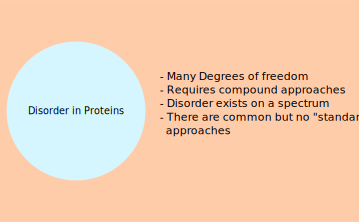
\includegraphics[scale=0.3]{intro.png}
    \caption{Proteins with disorder lack a rigid structure and require specialized approaches.}
    \label{fig:intro}
\end{figure}
\end{frame}


\begin{frame}
\frametitle{Motivation}
Characterization of disorder in proteins is important as disordered proteins are involved in cellular signaling and regulation,\cite{wrightIntrinsicallyDisorderedProteins2015}
and are associated with human diseases, such as neurodegenerative disease, cardiovascular disease, amyloidoses, cancer, and diabetes.\cite{uverskyIntrinsicallyDisorderedProteins2008}
Although challenging, modern methods of characterizing proteins can provide new insights to crucial protein function human biological mechanisms. \cite{bonomiSimultaneousDeterminationProtein2018}.
\end{frame}


\begin{frame}
\frametitle{Characterization Requires a Combination of Theory and Experiment}
\begin{figure}
    \centering
    \includegraphics[scale=0.3]{two-methods.png}
    \caption{Two main ways of integrating theory and experiment \cite{thomasenConformationalEnsemblesIntrinsically2022}.}
    \label{fig:two-methods}
\end{figure}
\end{frame}


\begin{frame}
\frametitle{Roadmap}
\begin{figure}
    \centering
    \includegraphics[scale=0.35]{roadmap.png}
    \caption{Definition roadmap}
    \label{fig:roadmap}
\end{figure}
\end{frame}

\section{Conformational Ensembles}

\begin{frame}
\frametitle{A Concrete Construction of a Conformational Ensemble}
\begin{figure}
    \centering
    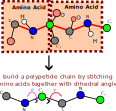
\includegraphics[scale=0.6]{dihedral-angles.png}
    \caption{A simple method of constructing a polypetide is to chain together amino acids.
    In this case, the only parameter would be the dihedral angles between amino acids \cite{ozenneFlexiblemeccanoToolGeneration2012}. }
    \label{fig:dihedral-angles}
\end{figure}
\end{frame}

\begin{frame}
\frametitle{A Concrete Construction of a Conformational Ensemble}
\begin{figure}
    \centering
    \includegraphics[scale=0.4]{concrete-ensemble.png}
    \caption{One can sample many dihedral pairs to construct an ensemble, such as in Flexible-Meccano \cite{ozenneFlexiblemeccanoToolGeneration2012}. }
    \label{fig:concrete-ensemble}
\end{figure}
\end{frame}

\begin{frame}
\frametitle{Define Biasing}
\begin{block}{Biasing}
    \begin{itemize}
        \item In the previous slides we sampled $\phi/\psi$ to construct an ensemble of polypeptides. 
        \item The practice of biasing is where experimental data is used to alter the way in which the sampling occurs to match the experimental data.
    \end{itemize}
\end{block}
\end{frame}

\begin{frame}
\frametitle{Define Weighting}
\begin{block}{Weighting and Reweighting}
    \begin{itemize}
        \item Another approach to conformational ensembles is to assign a weight to each conformation after sampling.
        \item Forward models are used to compute ensemble obeservables.
        \item The weights assigned to the conformations can be reweighted to better match experimental data.
    \end{itemize}
\end{block}
\end{frame}

\begin{frame}
\frametitle{Forward Models}
\begin{figure}
    \centering
    \includegraphics[scale=0.35]{forward-model.png}
    \caption{Forward models take a computed conformational ensemble and "forward" it to a physical obeservable.
    This is often used as a verification or as a biasing tool \cite{thomasenConformationalEnsemblesIntrinsically2022}, \cite{ozenneFlexiblemeccanoToolGeneration2012}. }
    \label{fig:forward-model}
\end{figure}
\end{frame}

\begin{frame}
\frametitle{Example of Forward Model}
\begin{block}{Residual Dipole Coupling}
    \begin{itemize}
        \item An example of an experimental measurment is residual dipole coupling (RDC).
        \item RDC is an ensemble averaged and time averaged measurement from nuclear magnetic resonance experiments \cite{marionIntroductionBiologicalNMR2013}.
        \item That being said, the time averaging is often ignored unless specialized methods are used \cite{thomasenConformationalEnsemblesIntrinsically2022}.
    \end{itemize}
\end{block}
\end{frame}

\begin{frame}
\frametitle{Example of Forward Model}
    For example, in the algorithm Flexible-Meccano, the RDCs for each conformer, (indexed by $j$) with axial and rhombic components $A_a$, $A_r$ of an alignment tensor $A$ are \cite{ozenneFlexiblemeccanoToolGeneration2012}:
    \begin{equation}\label{eq:rdc}
        D^j_{IS} = - \frac{\gamma_I \gamma_S \hbar \mu_0}{8 \pi^2 r^3_{IS}} \left [ A_a (3 \cos^2 \theta - 1) + \frac{3}{2} A_r \sin^2 \theta \cos (2 \phi) \right ]
    \end{equation}
\end{frame}

\begin{frame}
\frametitle{Example of Forward Model}
    The total RDC is calculated by averaging over the conformations in the ensemble \cite{ozenneFlexiblemeccanoToolGeneration2012}.
    \begin{equation}
        D_{IS} = \left \langle D_I{IS}^j \right \rangle
    \end{equation}
\end{frame}

\begin{frame}
\frametitle{Reweighting}
\begin{figure}
    \centering
    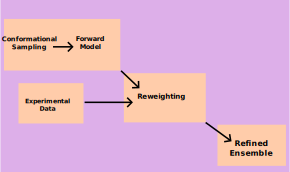
\includegraphics[scale=0.4]{reweighting.png}
    \caption{Diagram of reweighting method \cite{thomasenConformationalEnsemblesIntrinsically2022}. }
    \label{fig:reweighting}
\end{figure}
\end{frame}

\begin{frame}
\frametitle{Biasing}
\begin{figure}
    \centering
    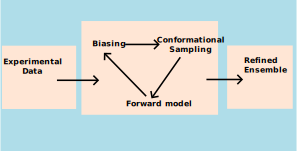
\includegraphics[scale=0.35]{biasing.png}
    \caption{Diagram of biasing method \cite{thomasenConformationalEnsemblesIntrinsically2022}. }
    \label{fig:biasing}
\end{figure}
\end{frame}

\section{A Note on Dynamics and Kinematics of Disordered Proteins}
\begin{frame}
\frametitle{Energy Landscapes}
\begin{figure}[h]
    \centering
    \includegraphics[scale=0.55]{energy-landscape.png}
    \caption{Transition rates and the protein's energy landscape.
        Low populated states often switch "slow" on a time scale of millisecons.
    Highly populated states often switch "fast" on the time scale of picoseconds \cite{bonomiDeterminationProteinStructural2019}. }
    \label{fig:min-bacteria}
\end{figure}
%Transition rates are the kinematics of the protein.
%Dynamics are based on the kinemetics. 
\end{frame}

\section{Wrapping Up}
\begin{frame}
    \frametitle{Perspectives on Protein Science}
    Below are perspectives on disordered proteins taken from various review papers:
    \begin{itemize}
        \item More robust/transferrable representations of structural ensembles \cite{bonomiDeterminationProteinStructural2019}
        \item Well defined threshold of "acceptable" results/accessible ways of comparing ensembles \cite{bonomiDeterminationProteinStructural2019}
        \item More transferrable and accurate force fields to help with integrative methods \cite{thomasenConformationalEnsemblesIntrinsically2022}
        \item Unified forward models: Developing forward models that are transferrable between proteins that do and do not have disorder \cite{thomasenConformationalEnsemblesIntrinsically2022}
    \end{itemize}
\end{frame}

\begin{frame}
    \frametitle{Conclusion}
    In this talk I reviewed the current state of protein science regarding how to handle disorder in proteins.
    Disorder is a many dimensional problem, which has necessitated the use of rigourous methods that combine computation with experiment.
    This has led to many interesting sub problems such as how to handle degeneracy and how to deal with the and quantification of errors.
    Most importantly though, the recent work done to characterize proteins may lead to many practical applications in treating human disease.

\end{frame}

\begin{frame}[allowframebreaks]
\frametitle{References}
\printbibliography
\end{frame}

\begin{frame}
    \frametitle{Thank you to:} 
    \begin{itemize}
        \item CU Prime: for funding me this semester
        \item Kevin Stenson: for supporting me over the summer and during this semester
        \item My girlfriends: Beth, Rae, June, and Maya: for emotionally supporting me through this time of rapid change
        \item My parents, Sherry and Rob: for making this "try" financially possible
        \item The queer and disabled community: for giving me a foundation of understanding for who I am and for creating spaces for me to feel safe
    \end{itemize}
\end{frame}

\begin{frame}
\frametitle{Questions?}
\end{frame}

\end{document}
